\documentclass{article}
\usepackage[T1]{fontenc}
\usepackage[a4paper,margin=2.5cm]{geometry}
\usepackage{amsmath}
\usepackage{pgfplots}
\pgfplotsset{compat=1.16}

\title{Week 11 Homework}
\date{}

\begin{document}
\maketitle

\section*{Question 1}

we have two identical pendulums, each with mass $m$ and length $l$. the spring has spring constant $k$ and is at equilibrium when $\theta_1=\theta_2=0$.

\subsection*{(a)}

the potential energy comes from gravity and the spring.

for each pendulum, the gravitational potential energy relative to its lowest point is

\[
V_g=mgl(1-\cos\theta).
\]

so for both pendulums,

\[
V_g=mgl(1-\cos\theta_1)+mgl(1-\cos\theta_2).
\]

for small angles, the horizontal displacement of each mass is approximately $l\theta$. therefore, the change in the spring's length is approximately

\[
\Delta x=l\theta_2-l\theta_1
=l(\theta_2-\theta_1).
\]

the spring potential energy is

\[
V_s=\frac{1}{2}k(\Delta x)^2
\]

so,

\[
V_s=\frac{1}{2}kl^2(\theta_2-\theta_1)^2.
\]

the total potential energy is therefore

\[
V=mgl(1-\cos\theta_1)+mgl(1-\cos\theta_2)
+\frac{1}{2}kl^2(\theta_2-\theta_1)^2.
\]

using the small-angle approximation $1-\cos\theta\approx\theta^2/2$,

\[
\boxed{
V\approx\frac{1}{2}mgl\theta_1^2
+\frac{1}{2}mgl\theta_2^2
+\frac{1}{2}kl^2(\theta_2-\theta_1)^2
}
\]

\subsection*{(b)}

the speed of each mass is $v=l\dot{\theta}$, so its kinetic energy is

\[
T=\frac{1}{2}mv^2
=\frac{1}{2}ml^2\dot{\theta}^{\,2}.
\]

adding the kinetic energies of both pendulums gives

\[
\boxed{
T=\frac{1}{2}ml^2\dot{\theta}_1^{\,2}
+\frac{1}{2}ml^2\dot{\theta}_2^{\,2}
}
\]

\subsection*{(c)}

the Lagrangian is

\[
L=T-V.
\]

we use the Euler--Lagrange equation for each angle,

\[
\frac{d}{dt}\left(\frac{\partial L}{\partial\dot{\theta_i}}\right)
-\frac{\partial L}{\partial\theta_i}=0.
\]

for $\theta_1$,

\[
\frac{\partial L}{\partial\dot{\theta}_1}
=ml^2\dot{\theta}_1
\]

and

\[
\frac{d}{dt}\left(\frac{\partial L}{\partial\dot{\theta}_1}\right)
=ml^2\ddot{\theta}_1.
\]

using the small-angle potential energy,

\[
\frac{\partial V}{\partial\theta_1}
=mgl\theta_1+kl^2(\theta_1-\theta_2).
\]

therefore,

\[
ml^2\ddot{\theta}_1+mgl\theta_1
+kl^2(\theta_1-\theta_2)=0.
\]

dividing by $ml^2$,

\[
\boxed{
\ddot{\theta}_1+\frac{g}{l}\theta_1
+\frac{k}{m}(\theta_1-\theta_2)=0
}
\]

similarly, for $\theta_2$,

\[
\frac{\partial V}{\partial\theta_2}
=mgl\theta_2+kl^2(\theta_2-\theta_1).
\]

so,

\[
ml^2\ddot{\theta}_2+mgl\theta_2
+kl^2(\theta_2-\theta_1)=0.
\]

dividing by $ml^2$ gives

\[
\boxed{
\ddot{\theta}_2+\frac{g}{l}\theta_2
+\frac{k}{m}(\theta_2-\theta_1)=0
}
\]

these equations show that the motion of each pendulum depends on the angle of the other pendulum because of the spring.

\subsection*{(d)}

for the symmetric mode, both pendulums move together, so

\[
\theta_1=\theta_2.
\]

the spring is not stretched in this mode. substituting $\theta_1=\theta_2$ into the first equation gives

\[
\ddot{\theta}_1+\frac{g}{l}\theta_1=0.
\]

comparing this with $\ddot{\theta}+\omega^2\theta=0$ gives

\[
\boxed{\omega_s=\sqrt{\frac{g}{l}}}.
\]

for the antisymmetric mode, the pendulums move in opposite directions, so

\[
\theta_1=-\theta_2.
\]

substituting $\theta_2=-\theta_1$ into the first equation gives

\[
\ddot{\theta}_1+\frac{g}{l}\theta_1
+\frac{k}{m}(2\theta_1)=0.
\]

therefore,

\[
\ddot{\theta}_1+
\left(\frac{g}{l}+\frac{2k}{m}\right)\theta_1=0.
\]

hence,

\[
\boxed{\omega_a=\sqrt{\frac{g}{l}+\frac{2k}{m}}}.
\]

the antisymmetric frequency is higher because the spring is stretched and compressed during this mode.

\subsection*{(e)}

the sketch has $k$ on the horizontal axis and $\omega$ on the vertical axis.

\begin{center}
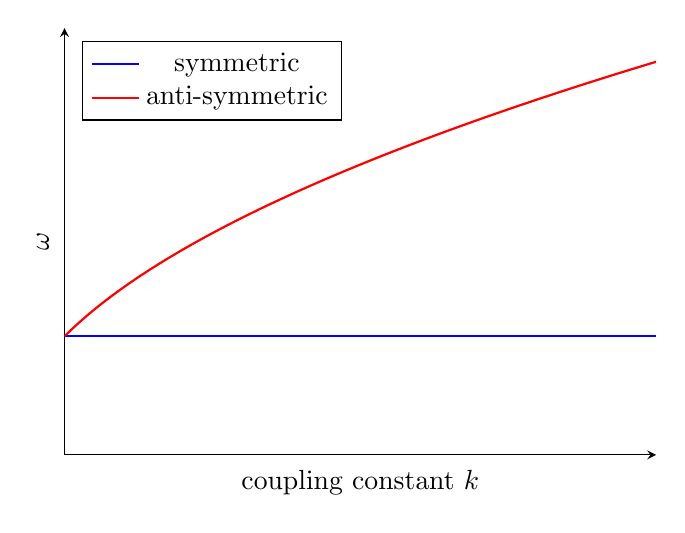
\begin{tikzpicture}
\begin{axis}[
  width=0.75\textwidth, height=7cm,
  xlabel={coupling constant $k$}, ylabel={$\omega$},
  xtick=\empty, ytick=\empty,
  axis lines=left, domain=0:5, samples=100,
  ymin=0, ymax=3.6, legend pos=north west
]
\addplot[blue, thick] {1};
\addlegendentry{symmetric}
\addplot[red, thick] {sqrt(1+2*x)};
\addlegendentry{anti-symmetric}
\end{axis}
\end{tikzpicture}
\end{center}

\section*{Question 2}

we have two masses $m_1$ and $m_2$ connected by a spring with spring constant $k$. there are no fixed ends, so the whole system can move together.

\subsection*{(a)}

the kinetic energy is

\[
T=\frac{1}{2}m_1\dot{x}_1^2
+\frac{1}{2}m_2\dot{x}_2^2.
\]

the spring extension is $x_2-x_1$, so the potential energy is

\[
V=\frac{1}{2}k(x_2-x_1)^2.
\]

the Lagrangian is $L=T-V$.

for $x_1$, the Euler--Lagrange equation gives

\[
m_1\ddot{x}_1=-k(x_1-x_2),
\]

or

\[
\boxed{m_1\ddot{x}_1+kx_1-kx_2=0}.
\]

for $x_2$,

\[
m_2\ddot{x}_2=-k(x_2-x_1),
\]

so

\[
\boxed{m_2\ddot{x}_2-kx_1+kx_2=0}.
\]

\subsection*{(b)}

we can write the equations in matrix form as

\[
\begin{pmatrix}
m_1&0\\
0&m_2
\end{pmatrix}
\begin{pmatrix}
\ddot{x}_1\\
\ddot{x}_2
\end{pmatrix}
+
\begin{pmatrix}
k&-k\\
-k&k
\end{pmatrix}
\begin{pmatrix}
x_1\\
x_2
\end{pmatrix}
=
\begin{pmatrix}
0\\
0
\end{pmatrix}.
\]

for a normal mode, assume

\[
x_1=A_1e^{i\omega t},\qquad
x_2=A_2e^{i\omega t}.
\]

then $\ddot{x}_i=-\omega^2x_i$, giving

\[
\begin{pmatrix}
k-m_1\omega^2&-k\\
-k&k-m_2\omega^2
\end{pmatrix}
\begin{pmatrix}
A_1\\
A_2
\end{pmatrix}
=
\begin{pmatrix}
0\\
0
\end{pmatrix}.
\]

for a non-zero solution, the determinant must be zero:

\[
(k-m_1\omega^2)(k-m_2\omega^2)-k^2=0.
\]

expanding,

\[
k^2-k(m_1+m_2)\omega^2+m_1m_2\omega^4-k^2=0.
\]

so,

\[
\omega^2\left[m_1m_2\omega^2-k(m_1+m_2)\right]=0.
\]

there are two solutions:

\[
\omega_1=0
\]

and

\[
\omega_2^2=\frac{k(m_1+m_2)}{m_1m_2}.
\]

therefore,

\[
\boxed{\omega_1=0,\qquad
\omega_2=\sqrt{k\left(\frac{1}{m_1}+\frac{1}{m_2}\right)}}.
\]

\subsection*{(c)}

the reduced mass is

\[
m_r=\frac{m_1m_2}{m_1+m_2}.
\]

rearranging,

\[
\frac{1}{m_r}=\frac{m_1+m_2}{m_1m_2}
=\frac{1}{m_1}+\frac{1}{m_2}.
\]

so the non-zero frequency can be written as

\[
\boxed{\omega=\sqrt{\frac{k}{m_r}}}.
\]

this is the frequency of the masses moving relative to each other. when one mass moves one way, the other moves the opposite way, changing the spring extension.

the zero-frequency mode means both masses move together with the same displacement. the spring is not stretched, so there is no restoring force. this is translation of the whole system, not an oscillation.

\subsection*{(d)}

for the non-zero frequency,

\[
\omega^2=k\left(\frac{1}{m_1}+\frac{1}{m_2}\right).
\]

using the first row of the matrix equation,

\[
(k-m_1\omega^2)A_1-kA_2=0.
\]

substituting the frequency,

\[
\left[k-m_1k\left(\frac{1}{m_1}+\frac{1}{m_2}\right)\right]A_1-kA_2=0.
\]

simplifying,

\[
-\frac{km_1}{m_2}A_1-kA_2=0.
\]

dividing by $-k$,

\[
\frac{m_1}{m_2}A_1+A_2=0.
\]

therefore,

\[
A_2=-\frac{m_1}{m_2}A_1.
\]

one possible eigenvector is

\[
\boxed{
\begin{pmatrix}
A_1\\
A_2
\end{pmatrix}
\propto
\begin{pmatrix}
m_2\\
-m_1
\end{pmatrix}
}.
\]

the negative sign means the masses move in opposite directions, so they are out of phase. the amplitude ratio is

\[
\boxed{\frac{|A_2|}{|A_1|}=\frac{m_1}{m_2}}.
\]

the lighter mass has the larger amplitude.

\section*{Question 3}

the clock pendulum is a damped driven oscillator with $T = 2$ s, so $f = 0.50$ Hz. the weight is a second pendulum, weakly coupled to it, with $\omega_w = \sqrt{g/\ell}$. as the weight falls, $\ell$ increases and $\omega_w$ decreases.

at $\ell = 0.99$ m,
\[
T_w = 2\pi\sqrt{\frac{0.99}{9.81}} \approx 2.0 \text{ s}
\]
so the weight matches the clock pendulum and is driven at resonance. the two coupled oscillators have equal frequencies, so energy transfers from the clock pendulum to the weight. the clock pendulum loses amplitude until the escapement cannot drive it, and the weight hits the side of the case. this happens late in the week, in the night between Thursday and Friday.

\end{document}